\documentclass[a4paper,10pt]{article}
%\documentclass[a4paper,10pt]{scrartcl}

\usepackage[utf8]{inputenc}
\usepackage{amsmath}
\usepackage{pgfplots}
\usepackage{graphicx}

\title{HW-2}
\author{Chi Zhang}
\date{09/27/2015}

\pdfinfo{%
  /Title    (HW-2)
  /Author   (Chi Zhang)
  /Creator  ()
  /Producer ()
  /Subject  ()
  /Keywords (VLSI, homework, HW, HW2)
}

\begin{document}
\maketitle
\section*{Q1}
\subsection*{a}
As \begin{math}V_{GS} = V_{DD} - V_{OH}\end{math} and only when \begin{math}V_{OH} \leq V_{DD} - V_{Th}\end{math} could 
guarentee the transistor is turned on. And the maximum value is the output voltage before t = 0.
\begin{equation}
\begin{split}
 V_{OH} &= V_{DD} - V_{Th}\\
        &= V_{DD} - V_{T0} - \gamma(\sqrt{2|\phi_F| + V_{OH}} - \sqrt{2|\phi_F|)}\\
        &=
\end{split}
\end{equation}
\subsection*{c}
When \begin{math}t\rightarrow\infty\end{math},
\begin{equation}
\begin{split}
V_{out} &= I_{DSAT}R_{SW}\\
&= \frac{1}{2}\kappa[V_{DD} - V_{out} - V_{T0} - \gamma(\sqrt{2|\phi_F| + V_{out} } - \sqrt{2|\phi_F|})] ^2 R_{SW}\\
&=
\end{split}
\end{equation}
\subsection*{b}
As informed in the question, \begin{math}V_{Th}\end{math} is constant and is the average of its maximum and minimum, which is
\begin{equation}
\begin{split}
V_{Th} &= V_{T0} + \frac{1}{2}\gamma(\sqrt{2|\phi_F| + V_{OH}} + \sqrt{2|\phi_F| + V_{OH}/2}) -\gamma\sqrt{2|\phi_F|}\\
&=
\end{split}
\end{equation}
As \begin{math}V_{out} = V_{OH} \rightarrow V_{OH}/2\end{math}, \begin{math}V_{DS} = V_{DD} - V_{OH} \rightarrow V_{DD} -
V_{OH}/2\end{math}. Thus,
\begin{equation}
\begin{split}
R_{eq} &= \frac{1}{2}\left[ \frac{V_{DD} - V_{OH}}{\frac{1}{2}\kappa(V_{DD}-V_{OH}-V_{Th}) ^2} + \frac{V_{DD} - V_{OH}/2}{\frac{1}{2}\kappa(V_{DD}-V_{OH}/2-V_{Th}) ^2}\right]\\
&= \frac{V_{DD} - V_{OH}}{\kappa(V_{DD}-V_{OH}-V_{Th}) ^2} + \frac{V_{DD} - V_{OH}/2}{\kappa(V_{DD}-V_{OH}/2-V_{Th}) ^2}\\
&=
\end{split}
\end{equation}

\section*{Q2}
\begin{equation}
\begin{split}
V_X =& V_{DD} - I_{SD}R_1\\
=& V_{DD} + \frac{1}{2}\kappa\frac{W}{L}(V_X-V_{in}+V_{T0})^2 (1+\lambda V_X)R_1\\
=& 
\end{split}
\end{equation}
\subsection*{a}
\subsection*{b}
\begin{equation}
\frac{W}{L} = 3.24
\end{equation}

\section*{Q3}
\subsection*{a}
\begin{equation}
\begin{split}
t_{pLH} &= R_{eq}C_L ln\frac{V_{DD}}{V_{DD} - V_{out}}\\
&= R_{eq}C_L ln\frac{2V_{DD}}{V_{DD} + V_{Tn}}\\
&= \frac{3V_{DD}R_{eq}C_{L}}{2\kappa\frac{W}{L}(V_{DD} - V_{Tn})^2} (1-\frac{5}{6} \lambda V_{DD})
ln\frac{2V_{DD}}{V_{DD}+V_{Tn}}\\
&=
\end{split}
\end{equation}
\subsection*{b}
\begin{equation}
\begin{split}
\Delta t_{pLH} &= 0.69R_{eq}C_0 W_0\\
&= t_0
\end{split}
\end{equation}
\subsection*{c}
\begin{equation}
\begin{split}
t_{pHL} &= 0.69RC_L\\
& = 1.735 \times 10^{-6} (s)
\end{split}
\end{equation}
\subsection*{d}
With \begin{math}\beta_n = \beta_p\end{math}, and \begin{math}|\gamma_n| = |\gamma_p|\end{math} with 
\begin{math}|\lambda_n| = |\lambda_p|\end{math} from the table coming with questions.
\begin{math}\frac{t_{pLH, n}}{t_{pLH, p}}\end{math} becomes,
\begin{equation}
 \begin{split}
  \frac{t_{pLH, n}}{t_{pLH, p}} &= \frac{R_{eq, n}}{R_{eq, p}}\frac{ln\frac{2V_{DD}}{V_{DD} + V_{Tn}}}{ln\frac{2V_{DD}}{V_{DD} + 
  V_{Tp, 0}}} \\
  &= \frac{(V_{DD}-V_{Tp, 0})^2 (1-\frac{5}{6}\lambda_n V_{DD})ln\frac{2V_{DD}}{V_{DD} + V_{Tn}}}
  {(V_{DD}-V_{Tn})^2 (1-\frac{5}{6}\lambda_p V_{DD})ln\frac{2V_{DD}}{V_{DD} +V_{Tp, 0}}}
 \end{split}
\end{equation}
\section*{Q4}
\subsection*{a}
For \begin{math}V_{M} = 0.5V_{DD}\end{math}, \begin{math}\frac{W_n}{W_p} = \frac{90}{127.50575} \approx \frac{90}{127.5}\end{math}.\\
(((The following table need to be ploted!!!)))\\
\begin{tabular}{c|c}
 90/90	&	0.5576\\
 90/100	&	0.5715\\
 90/110	&	0.5819\\
 90/120	&	0.5925\\
 90/127.5	&	0.6\\
 90/140	&	0.6116\\
 90/150	&	0.6202\\
 90/160	&	0.6283\\
 90/170	&	0.6357\\
\end{tabular}
\subsection*{b}
For high-to-low delay equals low-to-high delay, \begin{math}\frac{W_n}{W_p} = \frac{90}{135.75}\end{math}.\\
\begin{figure}
 \centering
 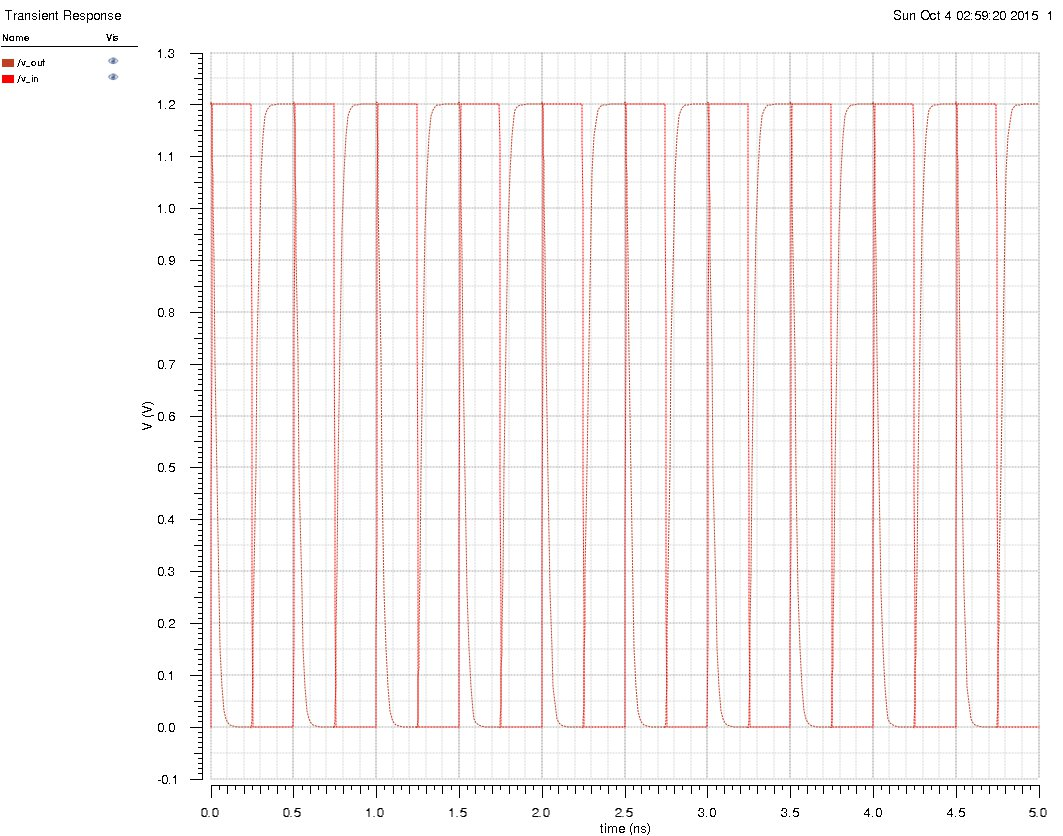
\includegraphics[width=10cm]{Q4_b.jpg}
 \caption{Q4\_b}
\end{figure}

\subsection*{c}
(((The following table need to be ploted)))\\
\begin{tabular}{c c}
 D\_input(ps)	&	t\_pHL\\
 0.1		&	n/c\\
 50		&	n/c\\
 100		&	n/c\\
 150		&	n/c\\
 200		&	n/c\\
 500		&	n/c\\
\end{tabular}


\end{document}
